\section{Methodology}
% In order to discover the preferences of different stakeholders, semi-structured interviews were conducted using example explanations \cite{garcia2018mixed}. During these semi-structured interviews, the participants were asked to answer substantive questions based on the provided explanations, as well as questions to indicate what aspects of different explanations they prefer. These substantive questions were used to gauge their understanding of the explanations. This is important, as previous research found that preference and understanding do not necessarily go hand in hand \cite{szymanski2021visual}.

In order to discover the preferences of different stakeholders, semi-structured interviews were conducted using example explanations \cite{garcia2018mixed}. During these semi-structured interviews, the participants were asked to answer substantive questions based on the provided explanations, as well as questions to indicate what aspects of different explanations they prefer. These substantive questions were used to gauge their understanding of the explanations. This is important, as previous research found that preference and understanding do not necessarily go hand in hand \cite{szymanski2021visual}. In our study, we are interested in particular in highlighting the specific explanation preferences of the specific stakeholders. Hence, we decompose our main research question into the following three sub-questions:

\begin{description}
    \item[SQ1:] What type of explanation is most suited for the different stakeholders?
    \item[SQ2:] What aspects of explanations make them more suited for each stakeholder?
    \item[SQ3:] In what way can different explanation types be combined to make them useful for each stakeholder?
\end{description}


\subsection{Hypotheses}

In this study, we consider three different explanation types (see Section \ref{sec:explanation_types}): (i) graph-based explanations; (ii) Textual explanations; and (iii) Feature attribution explanations. While the graph-based explanations will most likely be best suited for individuals with a fair amount of prior AI knowledge, the general lay users will probably gravitate towards the textual explanations, as those are both expressive and fairly easy to process \cite{purificato2021evaluating}. Considering the graph-based explanations contain the most information, but are expected to be the hardest to read, and the opposite holds for the feature attributions, the textual explanations are likely to strike a good balance between the two. These considerations lead us to formulate two hypotheses related to the \textbf{SQ1}:

\begin{itemize}
    \item \textbf{H1a}: \textit{The graph-based explanation will be best suited for individuals with prior AI knowledge.}
    \item \textbf{H1b}: \textit{The textual explanations will be best suited for individuals without prior AI knowledge.}    
\end{itemize}

Furthermore, we considered that feature attribution maps are usually the easiest and fastest way to get an overview of the model's rationale, but at the same time, they have a fairly limited extent \cite{szymanski2021visual}. The textual explanation will be more complex and take more time to process, but will provide a more comprehensive explanation in return. Lastly, the graph-based explanations will take the longest to process and might be difficult to interpret by themselves, but will contain the most complete explanation as a result. We then expect differences among the stakeholders, and formulate the following hypothesis related to the \textbf{SQ2}:

\begin{itemize}
    \item \textbf{H2}: \textit{The different stakeholders (candidates, companies, and recruiters) will have different preferences related to the explanation types.}   
\end{itemize}

Finally, we considered that explanations consisting of a single type may be either too limited in their content, or too difficult to interpret. This problem can be addressed by incorporating aspects from different types into a single explanation type \cite{szymanski2021visual}. For example, textual explanations can help in assisting the stakeholders in how to read the graph-based explanation. Furthermore, the feature attribution map can be useful when the stakeholder prefers to get a good (albeit limited) overview at a glance \cite{schellingerhout2022explainable}. We further hypothesize then that also regarding the preferences in terms of combining basic explanations into hybrid strategies, the stakeholders will have differences. Hence, we formulated the following hypothesis related to the \textbf{SQ3}:

\begin{itemize}
    \item \textbf{H3}: \textit{The different stakeholders (candidates, companies, and recruiters) will have different preferences on how to combine explanation types to obtain a hybrid explanation.}

\end{itemize}


\subsection{Semi-structured interview guide}
A comprehensive guide was created to conduct the semi-structured interviews (\cref{app:interview_guide}). However, this guide is susceptible to possible biases, ambiguities, incorrect assumptions about prior knowledge, etc. Thus, during the interviews, we dedicated time specifically to determining the quality of the questions in order to update, and eventually validate them. The questions in the interview guide were based upon previous works \cite{chen2005trust,cramer2008effects,kleinerman2018providing,pu2011user}, but required validation for a multi-stakeholder scenario. In addition to validating the interview guide, the interviews also allowed the stakeholders to co-design the explanation representations to fit their needs. The interviews were conducted with a small sample of the different stakeholders ($n = 2$ for each stakeholder type) to verify the adequacy of the explanations and the guide for each group individually. Considering the fact that each participant was interviewed three times (once for each explanation type), we collected a large amount of data per participant. Due to the richness of this data, the relatively small sample size still allowed us to perform an in-depth analysis for each stakeholder type. Previous works also indicates that a small sample can be sufficient in qualitative analysis, as long as the data itself is of high enough quality \cite{dworkin2012sample,morse2000determining}. Note that the user study was approved by the ethical committee of our institution.\footnote{Ethical Review Committee Inner City faculties (Maastricht University)}

% \subsection{Co-design session}
% After the pilot study has been conducted, the interview guide will be used to conduct a co-design study with the stakeholders. Based on the co-design study, it will be possible to determine which explanation types are most satisfactory and effective for each stakeholder. Each of the three main stakeholders will be represented by 10 individuals in order to have a sufficient sample. These individuals will have different levels of experience and be sampled from different industries in order to decrease potential bias within specific industries/experience levels. Each participant will be interviewed about each explanation type, i.e., the study will be within-subject. 

\subsection{Data \& model}
The explanations used for the interviews were generated using a job recommendation dataset provided by Zhaopin.\footnote{\url{https://tianchi.aliyun.com/dataset/31623/}} This dataset contains information on 4.78 million vacancies, 4.5 thousand candidates, and 700 thousand recorded interactions between the two. For candidates, the dataset stores information such as their degree(s), location, current and desired industry, skill set, and experience. For vacancies, features such as the job description, job title, salary, (sub-)type, required education, location, and starting date were recorded. The interactions between candidates and vacancies consist of four stages: no interaction, browsed, delivered, and satisfied. Considering the data in the dataset was exclusively in Mandarin Chinese, all unstructured data was automatically translated to English using deep-translator.\footnote{\url{https://pypi.org/project/deep-translator/}}

These three different tables were combined together into a single knowledge graph, wherein candidates, vacancies, and categorical features formed the set of nodes. The edges consisted of relations between these nodes, such as candidates interacting with vacancies or vacancies being of a specific (sub-)type. This single, large knowledge graph was then converted to individual sub-graphs between candidates and vacancies that had interacted (positives), and between those who had not interacted (negatives) using the k random walks algorithm \cite{lovasz1993random}. Each of these sub-graphs therefore could be given a score from 0 (no interaction), to 3 (satisfied), which allowed us to treat the task as a ranking problem based on sub-graph prediction.

The explainable model was based on the graph attention network (GAT) \cite{velivckovic2017graph}, implemented using PyTorch geometric.\footnote{\url{https://www.pyg.org/}} Considering performance was not the goal of this research, we opted for a straightforward architecture consisting of a single GATv2Conv-layer, followed by two separate GATv2Conv-layers - one for the company-side prediction and explanation, and one for the candidate-side prediction and explanation. Both these layers were followed by their own respective fully-connected layer, which provided the company- and candidate-side prediction score. The harmonic mean of these two scores was then considered the final `matching score'. Optimization was done using the Adam optimizer \cite{kingma2014adam} (learning rate $= 1 * 10^{-3}$) with LambdaRank loss based on normalized Discounted Cumulative Gain @ 10 (nDCG@10) \cite{burges2006learning}. Hyperparameter tuning was done using grid search going over different configurations of hyperparameters \cite{liashchynskyi2019grid}. Since our aim was not to get state-of-the-art performance, the number of different configurations tested was fairly limited. Even so, the optimal configuration led to an nDCG@10 of 0.2638 (\cref{app:hyperparameters}).

Considering the goal of our research was not to evaluate the explanation quality of the specific model, but rather to investigate stakeholder preferences in general, the examples used during the interviews were manually selected based on the following criteria: graph size, perceived sensibility, and accessibility of the industry for evaluation. By sticking to seemingly sensible explanations that did not require knowledge of the specific industry at hand, we aimed to make the stakeholders' evaluation dependent solely on the representation of the explanation, rather than the quality of the model's explanations in general. 

\subsection{Explanation types}
\label{sec:explanation_types}
The explanation types that were examined in this study were the following:

% Validation of questions using Factor Analysis
\begin{description}
    \item[Graph:] a visualization of paths in a knowledge graph. In our case, this consists of (a sub-set of) the paths within the candidate-vacancy sub-graph, weighted by the importance ascribed to them by the model (\cref{fig:paths});
    \item[Textual:] a short text that explains which features contributed to the recommendation in what way. The textual explanations are generated using a large language model (in this case, ChatGPT \cite{openai2022chatgpt}), which is given the full graph explanation as input, and tasked to summarize it in an easy-to-read way (\cref{fig:textual}); 
    \item[Feature attribution:] a visualization (such as a bar chart) that shows which features were most important to the model when creating the explanation (\cref{fig:attribution}). This bar chart is also based on the paths within the knowledge graph - the sizes of the bars are calculated using the sum of incoming edge weights, similar to PageRank \cite{bianchini2005inside}.
    % \item[Hybrid:] a combination of the three above types. Concretely, a hybrid explanation consists of one or more visualizations supported by some explanatory text. 
\end{description}

\begin{figure}[th]
    \caption{An example of knowledge graph paths being used as an explanation for a recommendation.}
    \hspace{-1.25cm}
    \begin{subfigure}[b]{0.615\linewidth}
         \centering
         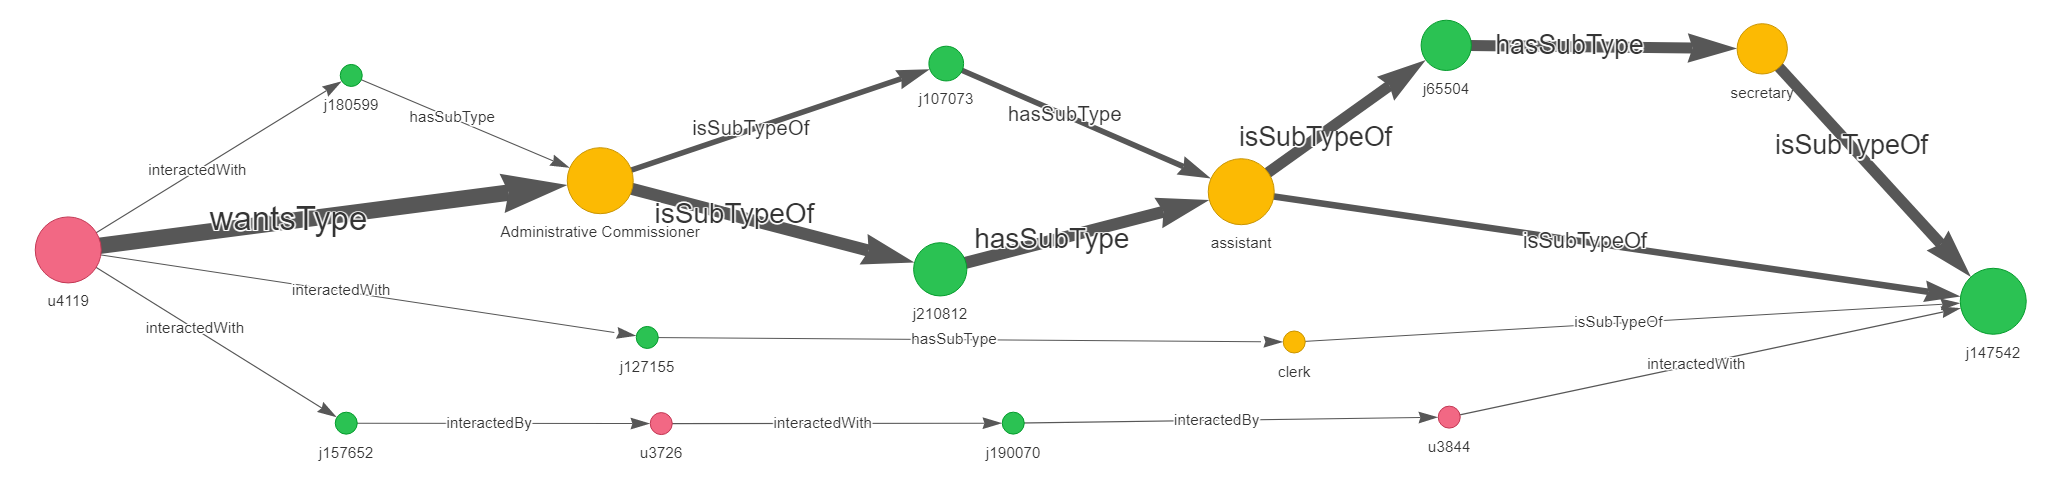
\includegraphics[width=\textwidth]{images/graph_candidate.png}
         \caption{Candidate-side graph}
         \label{fig:cand_side}
     \end{subfigure}
     \hfill
     \begin{subfigure}[b]{0.615\linewidth}
         \centering
         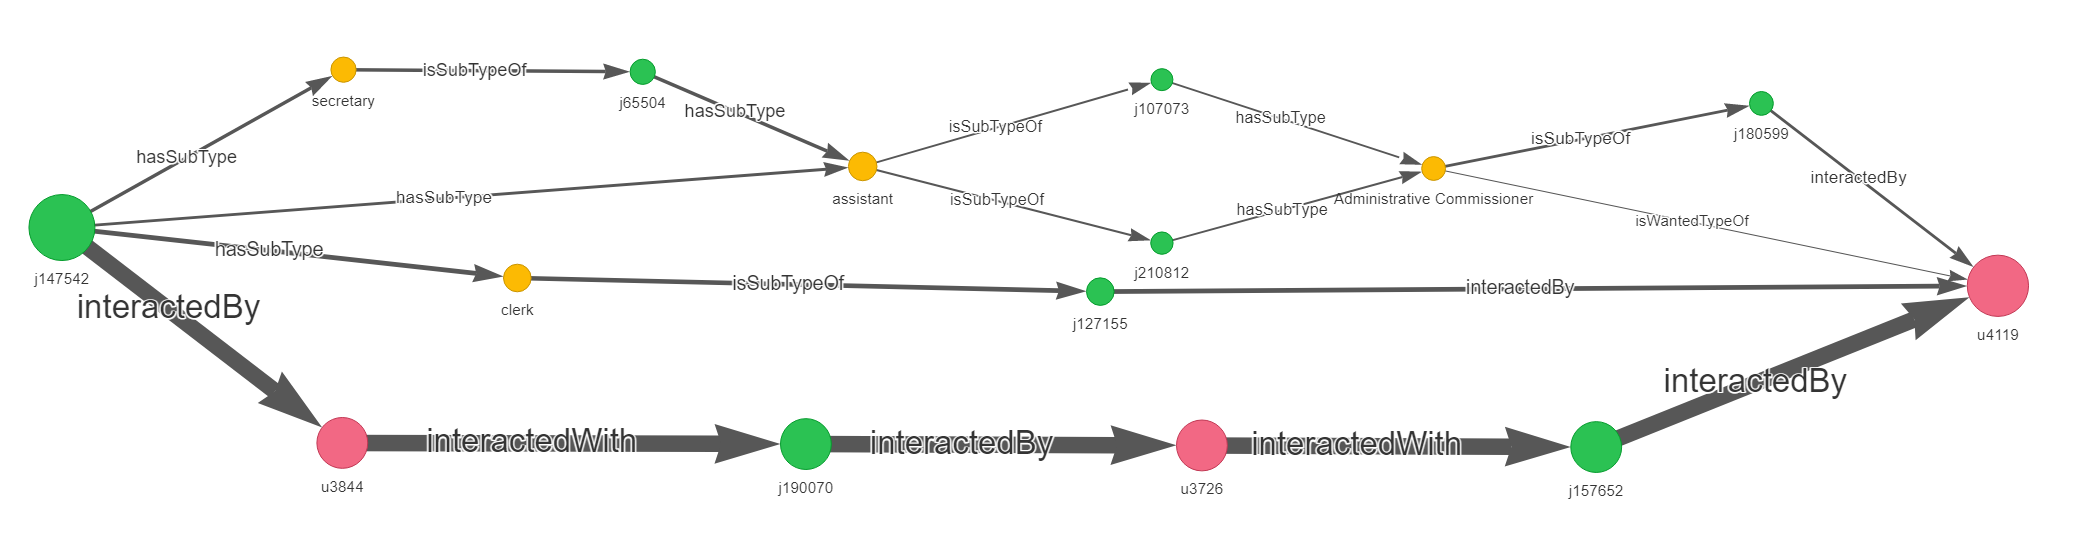
\includegraphics[width=\textwidth]{images/graph_company.png}
         \caption{Company-side graph}
         \label{fig:comp_side}
     \end{subfigure}
    \label{fig:paths}
\end{figure}

\newpage

\begingroup{
    \captionsetup{type=figure}
    \captionof{figure}{An example of a textual explanation used as an explanation for a recommendation}
    \fbox{\begin{minipage}{0.9\linewidth}
    The XAI model has analyzed various connections between jobs and users to determine if a particular user (\textcolor{xpink}{user 4119}) would be a good fit for a specific job (\textcolor{xgreen}{job 147542}). The model looked at the relationships between different jobs and users, as well as the importance of these relationships, to make its prediction.
    
    \vspace{0.1in}
    
    In this case, the model found that \textcolor{xpink}{user 4119} has a strong connection to the role of \textcolor{xyellow}{Administrative Commissioner}, and this connection is considered to be very important for explaining why \textcolor{xpink}{user 4119} would be a good match for \textcolor{xgreen}{job 147542}. Additionally, the model found that \textcolor{xgreen}{job 147542} has a connection to the role of \textcolor{xyellow}{secretary}, which is also considered important. The model also found that the \textcolor{xyellow}{Administrative Commissioner} role has a connection to the \textcolor{xyellow}{assistant} role, which in turn has a connection to the \textcolor{xyellow}{secretary} role and \textcolor{xgreen}{job 147542}.
    
    \vspace{0.1in}
    
    In summary, the XAI model determined that \textcolor{xpink}{user 4119} would be a good fit for \textcolor{xgreen}{job 147542} based on the strong connection between \textcolor{xpink}{user 4119} and the \textcolor{xyellow}{Administrative Commissioner} role, as well as the connections between the \textcolor{xyellow}{Administrative Commissioner} role, the \textcolor{xyellow}{assistant} role, the \textcolor{xyellow}{secretary} role, and \textcolor{xgreen}{job 147542}.
    \end{minipage}}
    \label{fig:textual}
}

\begin{figure}[bht]
    \caption{An example of a feature attribution map used as an explanation for a recommendation.}
    \centering
    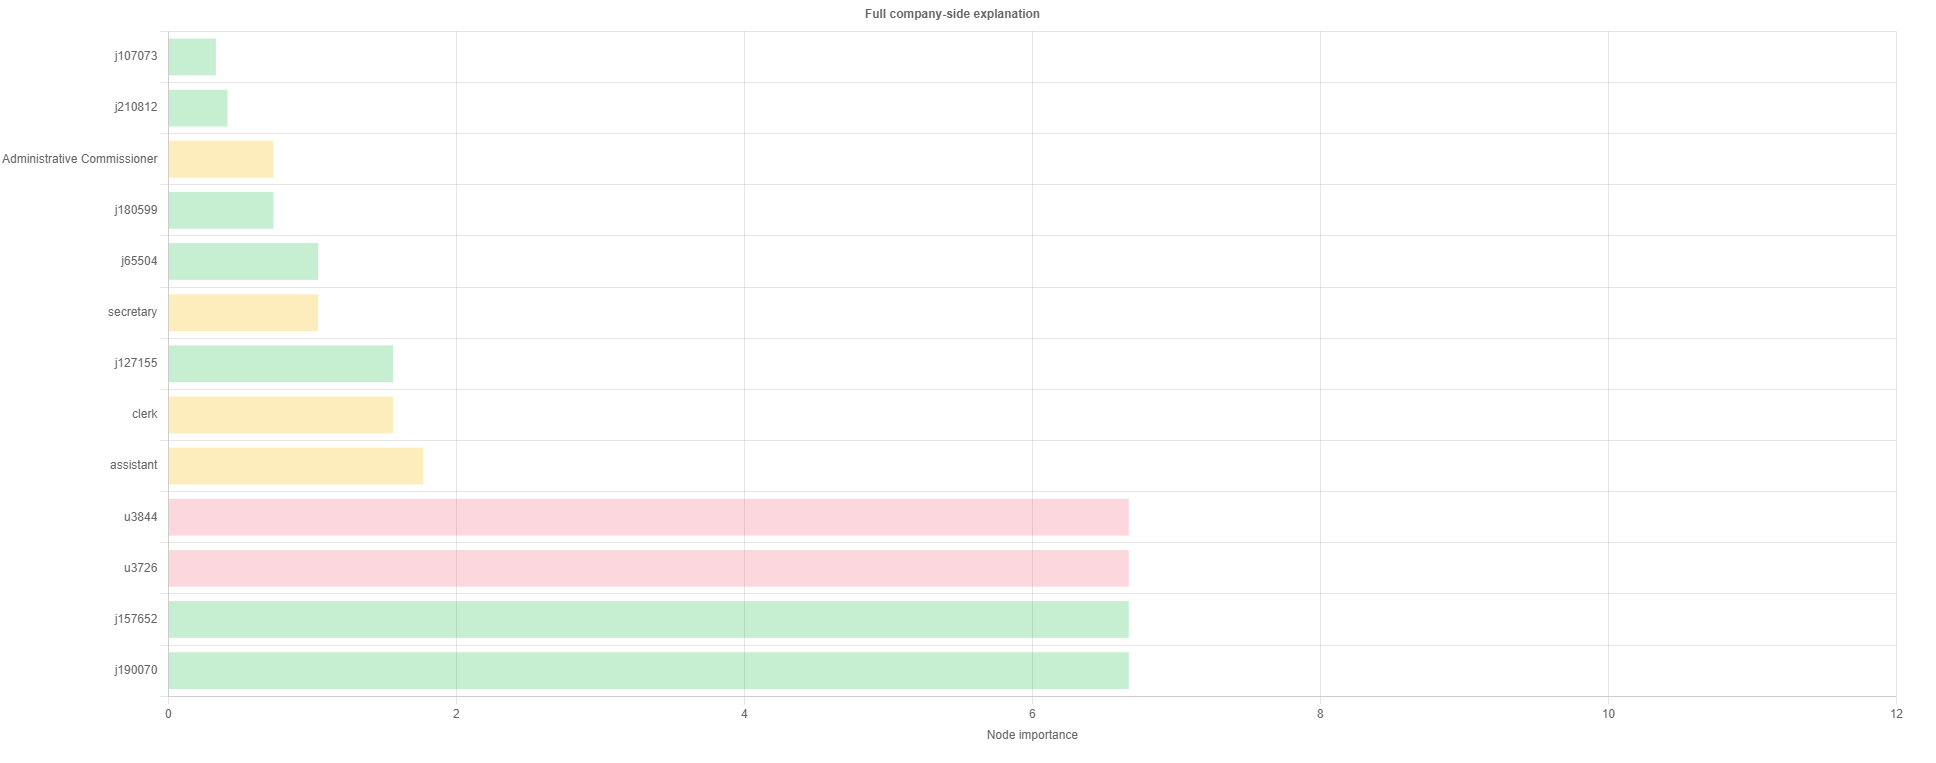
\includegraphics[width=\linewidth]{images/bar.png}
    \label{fig:attribution}
\end{figure}

% The participants will be questioned about all three explanation types once during the interview. The order in which the explanation types are shown will be randomized to minimize potential bias (as later explanations could develop an advantage due to participants getting more `experienced' with parsing them). As a result, each explanation type will have a total of 30 evaluations, split across the three stakeholder types. 


\subsection{Analysis}
The answers provided by the participants were analyzed using grounded theory (GT) \cite{walker2006grounded} using \textit{Atlas.ti}\footnote{\url{https://atlasti.com/}}. This process was done separately for each stakeholder type, in order to create distinct results for each type. We started by assigning manually-generated codes to individual statements made by the participants (open coding). These codes were then grouped together into distinct categories using axial coding to provide a higher-level overview of the complaints and preferences of each stakeholder type. Lastly, selective coding was conducted to combine each stakeholder type's categories into a single theory. The higher-level categories, as well as the theories, were then used to improve the prototypical explanation. 

\subsection{Participant demographics}
The participants were recruited through personal connections in collaboration with Randstad Groep Nederland\footnote{\url{https://www.randstad.nl/}}, the largest recruitment agency in the Netherlands. The sample consisted of 4 women and 2 men, of various ages ($\mu = 39.2, SD = 11.3, l=23, h=53$), with various backgrounds (tech, finance, healthcare, marketing, etc.). The participants had largely different levels of expertise w.r.t. AI, ranging from no knowledge whatsoever to a Bachelor's degree in a related field. Each interview took approximately one hour, and candidates were paid \euro{11,50} for their time. 
%NT: removing for anonymization
% - in line with Dutch minimum wage. 